  \section{Actividad Práctica}
    Se propone realizar las mediciones de potencias y factor de potencia en una carga reactiva, la cual 
    se trata de un tubo fluorescente común. Este mismo se encuentra prepardo junto a un circuito de medición
    que provee la cátedra. En la Figura~\ref{fig:CircuitoMedicion} se puede apreciar un esquema del mismo y una foto real.

    \begin{figure}[H]
      \centering
      \frame{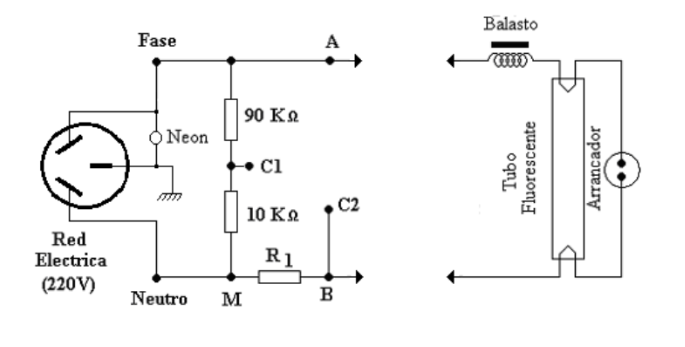
\includegraphics[width=0.8\textwidth]{Imagenes/ActividadPractica/EsquemaCircuito.png}}
      \caption{Circuito de medición propuesto por la cátedra.}
      \label{fig:CircuitoMedicion}
    \end{figure}
    
      \subsection{Medición de potencia activa y factor de potencia} 
  

      \subsection{Correción del factor de potencia}

